\section*{Exercises}

\begin{ex}
  Which of the following are quadratic forms?
  \begin{enumerate}
  \item $f_1(x,y,z) = (x+y+z)^2$.
  \item $f_2(x,y,z) = x^2 + y^2 + z^2$.
  \item $f_3(x,y,z) = (x+y)^2 + (x+z)^2 + (y+z)^2$.
  \item $f_4(x,y,z) = x^2 - y^2$.
  \item $f_5(x,y,z) = x^2 + 2xyz + (y+z)^2$.
  \item $f_6(x,y,z) = x(y+z)$.
  \item $f_7(x,y,z) = x^2y^2z^2$.
  \end{enumerate}
  \begin{sol}
    All of them except (e) and (g).
  \end{sol}
\end{ex}

\begin{ex}
  Find the coefficients of the quadratic form
  $f(x,y,z) = \vect{v}^T A\vect{v}$, where
  \begin{equation*}
    A = \begin{mymatrix}{rrr}
      0 &  1 &  2 \\
      1 & -3 & -4 \\
      2 & -4 &  5 \\
    \end{mymatrix}.
  \end{equation*}
\end{ex}

\begin{ex}
  Write the quadratic form
  \begin{equation*}
    f(x,y,z) = (x+y)^2 + 2(x-z)^2 + 3yz
  \end{equation*}
  in matrix form.
  \begin{sol}
    $f(x,y,z) = \vect{v}^T A\vect{v}$, where
    \begin{equation*}
      A = \begin{mymatrix}{ccc}
        3  &  1  & -2  \\
        1  &  1  & 1.5 \\
        -2 & 1.5 &  2  \\
      \end{mymatrix}.
    \end{equation*}
  \end{sol}
\end{ex}

\begin{ex}
  Apply the change of variables $x = u+2w$, $y = v$, $z = w-v$ to the
  quadratic form
  \begin{equation*}
    x^2 + 7y^2 + 5z^2 - 4xy - 4xz + 11yz.
  \end{equation*}
  \begin{sol}
    $3u^2 + v^2 + vw + w^2$.
  \end{sol}
\end{ex}

\begin{ex}
  Perform a change of variables so that the quadratic form
  $f(x,y) = 3x^2 - 2xy + 3y^2$ becomes diagonal.
  \begin{sol}
    $x=u+v$ and $y=u-v$ gives $f = 4u^2 + 8v^2$.
  \end{sol}
\end{ex}

\begin{ex}
  Diagonalize the quadratic form
  \begin{equation*}
    f(x,y,z) = 3x^2 + 3y^2 + 4z^2 + 2xz - 2yz.
  \end{equation*}
\end{ex}

\begin{ex}
  Find the principal axes of the following curves, and sketch them:
  \begin{enumerate}
  \item $x^2+\frac{1}{2}y^2=1$,
  \item $2x^2 + 4xy + 5y^2 = 1$.
  \item $3x^2 + 2xy + 3y^2 = 1$.
  \end{enumerate}
  \begin{sol}
    \begin{enumerate}
    \item Eigenvalues: $\eigenvar_1=1$, $\eigenvar_2=\frac{1}{2}$.
      Principal axes:
      $\vect{u}_1 = \begin{mymatrix}{r} 1 \\ 0 \end{mymatrix}$ and
      $\vect{u}_2 = \begin{mymatrix}{r} 0 \\ 1 \end{mymatrix}$.
      $\vect{u}_1$-intercept: $1$, $\vect{u}_2$-intercept: $\sqrt{2}$.
    \item Eigenvalues: $\eigenvar_1=1$, $\eigenvar_2=6$.
      Principal axes:
      $\vect{u}_1 = \frac{1}{\sqrt{5}}\begin{mymatrix}{r} 2 \\ -1 \end{mymatrix}$ and
      $\vect{u}_2 = \frac{1}{\sqrt{5}}\begin{mymatrix}{r} 1 \\ 2 \end{mymatrix}$.
      $\vect{u}_1$-intercept: $1$, $\vect{u}_2$-intercept: $\frac{1}{\sqrt{6}}$.
    \item Eigenvalues: $\eigenvar_1=2$, $\eigenvar_2=4$.
      Principal axes:
      $\vect{u}_1 = \frac{1}{\sqrt{2}}\begin{mymatrix}{r} 1 \\ -1 \end{mymatrix}$ and
      $\vect{u}_2 = \frac{1}{\sqrt{2}}\begin{mymatrix}{r} 1 \\ 1 \end{mymatrix}$.
      $\vect{u}_1$-intercept: $\frac{1}{\sqrt{2}}$, $\vect{u}_2$-intercept: $\frac{1}{2}$.
    \end{enumerate}
    \begin{equation*}
      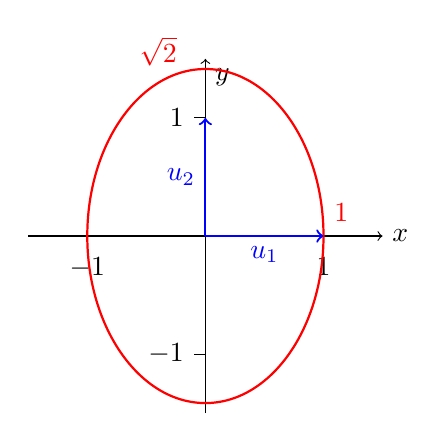
\begin{tikzpicture}[scale=1.5]
        \begin{scope}[color=black]
          \draw[->] (-1.5,0) -- (1.5,0) node[right] {$x$};
          \draw[->] (0,-1.5) -- (0,1.5) node[below right] {$y$};
          \draw (-1,0) -- +(0,-.1) node[below] {$-1$};
          \draw (1,0) -- +(0,-.1) node[below] {$1$};
          \draw (0,-1) -- +(-.1,0) node[left] {$-1$};
          \draw (0,1) -- +(-.1,0) node[left] {$1$};
        \end{scope}
        \begin{scope}[color=blue,cm={(1,0,0,1,(0,0))}]
          \draw[thick,red] (0,0) circle [x radius={1}, y radius={sqrt(2)}];
          \draw[red] (1,0) +(0.15,0.2) node {$1$};
          \draw[red] (0,{sqrt(2)}) +(-0.4,0.15) node {$\sqrt{2}$};
          \draw[thick,blue,->] (0,0) -- node[below] {$\vect{u}_1$} (1,0);
          \draw[thick,blue,->] (0,0) -- node[left] {$\vect{u}_2$} (0,1);
        \end{scope}
      \end{tikzpicture}
      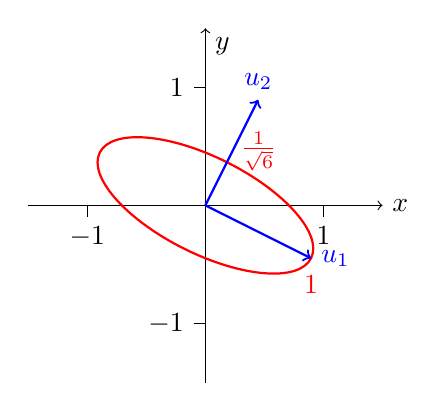
\begin{tikzpicture}[scale=1.5]
        \begin{scope}[color=black]
          \draw[->] (-1.5,0) -- (1.5,0) node[right] {$x$};
          \draw[->] (0,-1.5) -- (0,1.5) node[below right] {$y$};
          \draw (-1,0) -- +(0,-.1) node[below] {$-1$};
          \draw (1,0) -- +(0,-.1) node[below] {$1$};
          \draw (0,-1) -- +(-.1,0) node[left] {$-1$};
          \draw (0,1) -- +(-.1,0) node[left] {$1$};
        \end{scope}
        \begin{scope}[color=blue,cm={(2/sqrt(5),-1/sqrt(5),1/sqrt(5),2/sqrt(5),(0,0))}]
          \draw[thick,red] (0,0) circle [x radius={1}, y radius={1/sqrt(6)}];
          \draw[red] (1,0) +(0.1,-0.2) node {$1$};
          \draw[red] (0,{1/sqrt(6)}) +(0.2,0.2) node {$\frac{1}{\sqrt{6}}$};
          \draw[thick,blue,->] (0,0) -- (1,0) node[right] {$\vect{u}_1$};
          \draw[thick,blue,->] (0,0) -- (0,1) node[above] {$\vect{u}_2$};
        \end{scope}
      \end{tikzpicture}
      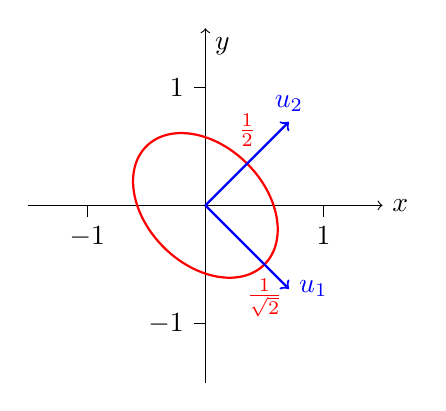
\begin{tikzpicture}[scale=1.5]
        \begin{scope}[color=black]
          \draw[->] (-1.5,0) -- (1.5,0) node[right] {$x$};
          \draw[->] (0,-1.5) -- (0,1.5) node[below right] {$y$};
          \draw (-1,0) -- +(0,-.1) node[below] {$-1$};
          \draw (1,0) -- +(0,-.1) node[below] {$1$};
          \draw (0,-1) -- +(-.1,0) node[left] {$-1$};
          \draw (0,1) -- +(-.1,0) node[left] {$1$};
        \end{scope}
        \begin{scope}[color=blue,cm={(1/sqrt(2),-1/sqrt(2),1/sqrt(2),1/sqrt(2),(0,0))}]
          \draw[thick,red] (0,0) circle [x radius={1/sqrt(2)}, y radius={1/2}];
          \draw[red] ({1/sqrt(2)},0) +(0.2,-0.2) node {$\frac{1}{\sqrt{2}}$};
          \draw[red] (0,{1/2}) +(-0.2,0.2) node {$\frac{1}{2}$};
          \draw[thick,blue,->] (0,0) -- (1,0) node[right] {$\vect{u}_1$};
          \draw[thick,blue,->] (0,0) -- (0,1) node[above] {$\vect{u}_2$};
        \end{scope}
      \end{tikzpicture}
    \end{equation*}
  \end{sol}
\end{ex}

\begin{ex}
  Find the principal axes of the ellipsoid
  $2x^2 + 2y^2 + 3z^2 + 2xz - 2yz$.
  \begin{sol}
    The principal axes are
    $\frac{1}{\sqrt{3}}\begin{mymatrix}{r} 1 \\ -1 \\ -1 \end{mymatrix}$,
    $\frac{1}{\sqrt{2}}\begin{mymatrix}{r} 1 \\ 1 \\ 0 \end{mymatrix}$,
    $\frac{1}{\sqrt{6}}\begin{mymatrix}{r} 1 \\ -1 \\ 2 \end{mymatrix}$.
  \end{sol}
\end{ex}

